% \date{May 14, 2024}
% \author{Deralive}
% \title{华东师范大学软件学院实验报告模板}
% 注意事项:编译两次,以确保目录、页码完整显示

\def\allfiles{}

%————————————多文件编译————————————%
% \ifx\allfiles\undefined
% 	    \begin{document}
% \else
% \fi

% Content

% \ifx\allfiles\undefined
% 	    \end{document}
% 	\else
% 	\fi
%—————————————————————————————————%

\documentclass[14pt,a4paper,UTF8,twoside]{article}

\usepackage{amsmath}
\usepackage{graphicx}
\usepackage{geometry} 
\usepackage{ctex}
\usepackage{booktabs} % 表格库
\usepackage{titlesec} % 标题库
\usepackage{fancyhdr} % 页眉页脚库
\usepackage{lastpage} % 页码数库
\usepackage{listings} % 代码块包
\usepackage{xcolor}
\usepackage[hidelinks]{hyperref}
\usepackage{tikz}
\usepackage{tikz-qtree}
\usepackage{fontspec} % 允许设置字体
\usepackage{unicode-math} % 允许数学公式使用特定字体
\usepackage{mwe}
\usepackage{zhlipsum} % 中文乱数文本
\usepackage{amsmath}
\usepackage{xcolor}
\usepackage{float} % 浮动体环境
\usepackage{subcaption} % 子图包
\usepackage{biblatex}
\usepackage{longtable}
\addbibresource{references.bib} % 指定你的.bib文件名称

\definecolor{mygreen}{rgb}{0,0.6,0}
\definecolor{mygray}{rgb}{0.5,0.5,0.5}
\definecolor{mymauve}{rgb}{0.58,0,0.82}

\date{} % 留空,以让编译时去除日期

%———————————————注意事项—————————————————%

% 1、如果编译显示失败,但没有错误信息,就是 filename.pdf 正在被占用
% 2、在文件夹中的终端使用 Windows > xelatex filename.tex 也可编译

%—————————————华东师范大学———————————————%

% 论文制作时须加页眉,页眉从中文摘要开始至论文末
% 偶数页码内容为:华东师范大学硕士学位论文,奇数页码内容为学位论文题目

%————————定义 \section 的标题样式————————%

% 注意:\chapter 等命令,内部使用的是 \thispagestyle{plain} 的排版格式
% 若需要自己加上页眉,实际是在用 \thispagestyle{fancy} 的排版格式
% 加上下面这一段指令,就能够让 \section 也使用 fancy 的排版格式
% 本质就是让目录、第一页也能够显示页眉、页脚

\fancypagestyle{plain}{
  \pagestyle{fancy}
}

\title{实验报告:Pintos安装} % 模板
\titleformat{\section}
    {\normalfont\bfseries\Large} % 字体大小、字体系列(\bfseries 为加粗)
    {\thesection}{1em}{}

% 设置章节的中文格式
\renewcommand\thesection{\chinese{section} \hspace{0pt}}
\renewcommand\thesubsection{\arabic{subsection} \hspace{0pt}}
% \renewcommand\thesubsubsection{\alph{subsubsection} \hspace{0pt}} % 字母编号
% \hspace{0pt} 是为了确保在章节编号和章节题目之间不要有空格,使得排版更为美观
    
%—————————————页面基础设置———————————————%

\geometry{left=10mm, right=10mm, top=20mm, bottom=20mm}

%————————————设置页眉、页脚——————————————%

\pagestyle{fancy} % 设置 plain style 的属性

% 设置页眉

\fancyhead[RE]{\leftmark} % Right Even 偶数页右侧显示章名 \leftmark 最高级别章名
\fancyhead[LO]{\rightmark} % Left Odd 奇数页左侧显示节名 \rightmark 第二级别节名
\fancyhead[C]{华东师范大学软件工程学院学生实践报告} % Center 居中显示
\fancyhead[LE,RO]{~\thepage~} % 在偶数页的左侧,奇数页的右侧显示页码
\renewcommand{\headrulewidth}{1.2pt} % 页眉与正文之间的水平线粗细

% 设置页脚:在每页的右下脚以斜体显示书名

\fancyfoot[RO,RE]{\it Lab Report By \LaTeX} % 使用意大利斜体显示
\renewcommand{\footrulewidth}{0.5pt} % 页脚水平线宽度

% 设置页码:在底部居中显示页码

\pagestyle{fancy}
\fancyfoot[C]{\kaishu 第 \thepage 页 \ 共 \pageref{LastPage} 页} % LastPage 需要二次编译以获取总页数

%——————————————代码块设置———————————————%

\lstset {
    backgroundcolor=\color{white},   % choose the background color; you must add \usepackage{color} or \usepackage{xcolor}
    basicstyle=\footnotesize,        % the size of the fonts that are used for the code
    breakatwhitespace=false,         % sets if automatic breaks should only happen at whitespace
    breaklines=true,                 % sets automatic line breaking
    captionpos=bl,                   % sets the caption-position to bottom
    commentstyle=\color{mygreen},    % comment style
    deletekeywords={...},            % if you want to delete keywords from the given language
    escapeinside={\%*}{*},           % if you want to add LaTeX within your code
    extendedchars=true,              % lets you use non-ASCII characters; for 8-bits encodings only, does not work with UTF-8
    frame=single,                    % adds a frame around the code
    keepspaces=true,                 % keeps spaces in text, useful for keeping indentation of code (possibly needs columns=flexible)
    keywordstyle=\color{blue},       % keyword style
    % language=Python,               % the language of the code
    morekeywords={*,...},            % if you want to add more keywords to the set
    numbers=left,                    % where to put the line-numbers; possible values are (none, left, right)
    numbersep=5pt,                   % how far the line-numbers are from the code
    numberstyle=\tiny\color{mygray}, % the style that is used for the line-numbers
    rulecolor=\color{black},         % if not set, the frame-color may be changed on line-breaks within not-black text (e.g. comments (green here))
    showspaces=false,                % show spaces everywhere adding particular underscores; it overrides 'showstringspaces'
    showstringspaces=false,          % underline spaces within strings only
    showtabs=false,                  % show tabs within strings adding particular underscores
    stepnumber=1,                    % the step between two line-numbers. If it's 1, each line will be numbered
    stringstyle=\color{orange},      % string literal style
    tabsize=2,                       % sets default tabsize to 2 spaces
    % title=Python Code              % show the filename of files included with \lstinputlisting; also try caption instead of title
}

% 注释掉的部分用于后续插入代码,参数可调整,格式如下:

% 1、直接插入
% \begin{lstlisting}[language = ? , title = { ? } ]
%       Your code here.
% \end{lstlisting}

% 2、文件插入
% \lstinputlisting[language = C , title = ?.c] {filename.c}

%———————————————字体设置————————————————%

% \setCJKmainfont{SimSun} % 设置正文罗马族的 CJK 字体
% \renewcommand{\normalsize}{\fontsize{12pt}{15pt}\selectfont} % 设置正文字号
\linespread{1.2}

%——————————————————————————————————————%

%———————————————超链接设置——————————————%

\hypersetup{
    pdfstartview=FitH, % 设置PDF文档打开时的初始视图为页面宽度适应窗口宽度(即页面水平适应)
    CJKbookmarks=true, % 用对CJK(中文、日文、韩文)字符的书签支持,确保这些字符在书签中正确显示
    bookmarksnumbered=true, % 书签带有章节编号。这对有章节编号的文档很有用
    bookmarksopen=true, % 文档打开时,书签树是展开的,方便查看所有书签
    colorlinks, % 启用彩色链接。这样,链接在PDF中会显示为彩色,而不是默认的方框
    pdfborder=001, % 设置PDF文档中链接的边框样式。001 表示链接周围没有边框,仅在单击时显示一个矩形
    linkcolor=blue, % 设置文档内部链接(如目录中的章节链接)的颜色为蓝色
    anchorcolor=blue, % 设置锚点链接(即目标在同一文档内的链接)的颜色为蓝色
    citecolor=blue, % 设置引用(如文献引用)的颜色为蓝色
}

%——————————————导言区结束,进入正文部分———————————————%

%——————————————————————————————————————%

\begin{document}

\maketitle

\begin{center} % \extracolsep{\fill} 拉伸到页面最大宽度前,保证居中显示

  \begin{tabular*}{\textwidth}{@{\extracolsep{\fill}} l  l  l }
    \hline
    课程名称:操作系统 &  年级:2023级本科  &  上机实践成绩:\ \ \ \ \ \ \ \ \ \ \ \ \ \\
    指导教师:张民 & 姓名:张梓卫 \\
    上机实践名称:Pintos安装 & 学号:10235101526 & 上机实践日期:\ \ \ \ \ \ \ \ \ \ \ \ \ \\
    上机实践编号:(1) & 组号: & 上机实践时间:\ \ \ \ \ \ \ \ \ \ \ \ \ \\
    \hline
  \end{tabular*}

\end{center}

\tableofcontents % 目录也需要二次编译

\section{实验目的}

本次实验为操作系统的第一次实验,目的是安装并运行 Pintos 操作系统,并熟悉操作系统的基本概念、原理和实践方法。
实验中,还对当下流行的 Docker 容器技术进行了实践,基于 PKU-OS 进行教学,让我们能够顺便熟悉 Linux 操作系统中的部分命令,为以后的开发打下基础。  

\section{内容与设计思想}

利用Docker在Windows 11上安装基于x86的PintOS(斯坦福大学)。

\section{使用环境}

使用 Docker v27.1.1 进行Pintos的安装实验,基于 Windows 11 操作系统使用 WSL2。

实验报告使用 \LaTeX 进行撰写,使用 Vim 编辑器进行文本编辑。

\section{实验过程与分析}

\subsection{使用Docker拉取镜像}

\begin{lstlisting}[language = bash, title = {拉取镜像}]
  docker run -it pkuflyingpig/pintos bash
\end{lstlisting}

\begin{figure} [H]
  \centering
  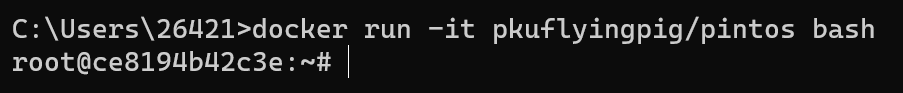
\includegraphics[width=0.8\textwidth]{img1/Dockerrun.png}
  \caption{拉取镜像后进入Docker容器}
  \label{fig:dockerrun}
\end{figure}

\subsection{从Github克隆代码}

注意,文档里写的这个无法拉取,需要使用SSH协议,需要在GitHub上设置SSH密钥。
\begin{lstlisting} [language = bash, title = {克隆代码}]
 > git clone hit@github.com:PKU-OS/pintos.git
\end{lstlisting}

所以使用了助教发送的新地址:
\begin{lstlisting} [language = bash, title = {克隆代码}]
  > git clone https://gitee.com/duerwuyi/pintos.git
\end{lstlisting}

Clone 代码结果如下:
\begin{figure} [H]
  \centering
  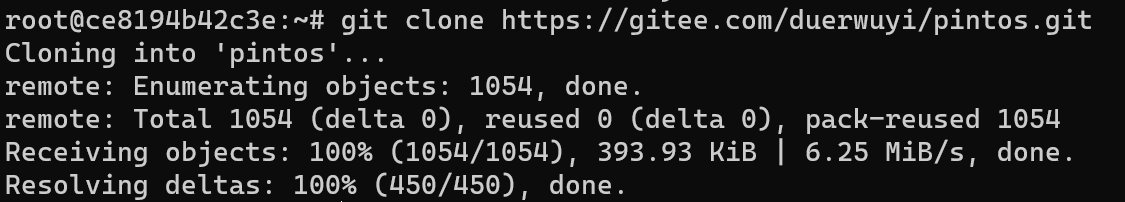
\includegraphics[width=0.6\textwidth]{img1/GitClone.png}
  \caption{克隆代码}
  \label{fig:clone}
\end{figure}

其中,Docker 中的 Log 显示了克隆的进度

\begin{figure} [H]
  \centering
  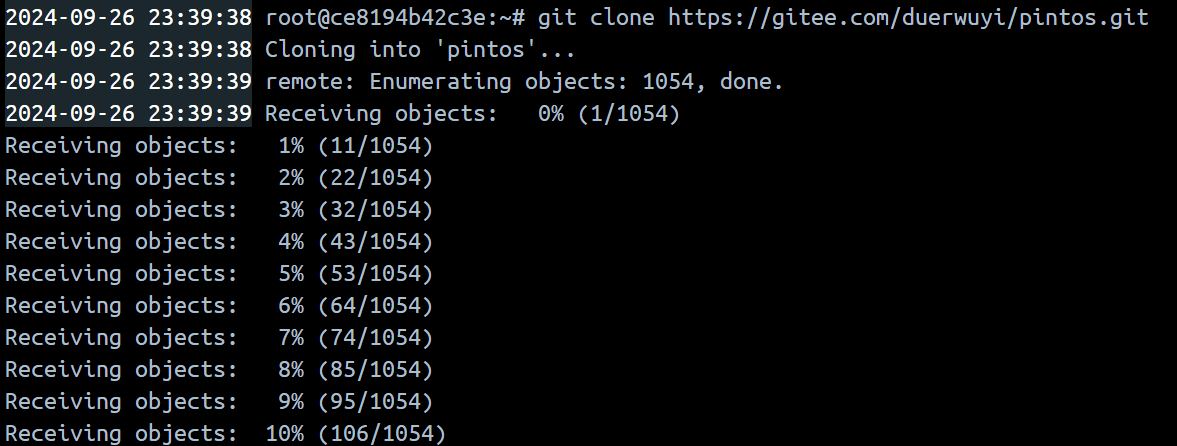
\includegraphics[width=0.6\textwidth]{img1/Schedule.png}
  \caption{克隆进度}
  \label{fig:schedule}
\end{figure}

\subsection{使用cd、pwd、ls命令等进入threads}

首先,对cd、pwd、ls等命令进行复习:

\subsubsection{cd 命令}
\begin{itemize} 
  \item cd 进入用户主目录; 
  \item cd \~{} 进入用户主目录; 
  \item cd - 返回进入此目录之前所在的目录; 
  \item cd .. 返回上级目录(若当前目录为“/”,则执行完后还在“/”;“..”为上级目录的意思); 
  \item cd ../.. 返回上两级目录; 
  \item cd !\$ 把上个命令的参数作为cd参数使用。 
\end{itemize}

\subsubsection{ls 命令}
\begin{itemize} 
  \item -a:列出目录下的所有文件,包括以.开头的隐藏文件; 
  \item -l:除了文件名之外,还将文件的权限、所有者、文件大小等信息详细列出来。 
\end{itemize} 

\subsubsection{pwd 命令}

全称 Print Working Directory,显示当前工作目录的完整路径。

\subsection{进入threads目录}

\begin{lstlisting} [language = bash, title = {进入threads目录}]
  > cd pintos
  > ls
  > cd src
  > ls
  > cd threads
\end{lstlisting}

\begin{figure} [H]
  \centering
  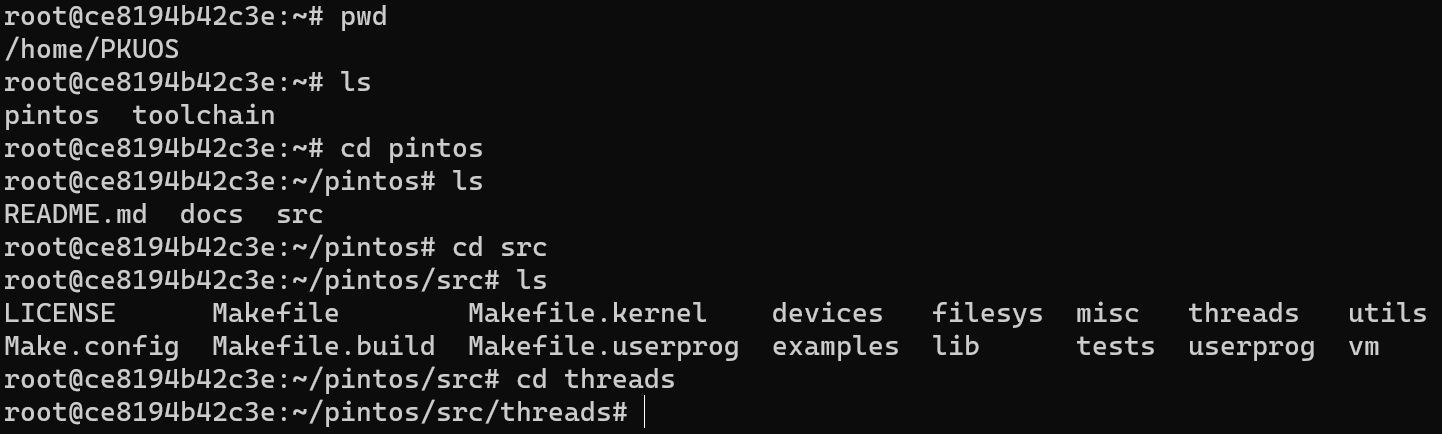
\includegraphics[width=0.6\textwidth]{img1/EnterThreads.png}
  \caption{进入threads目录}
  \label{fig:threads}
\end{figure}

这部分疯狂使用 \texttt{ls} 命令是为了在命令行中没有界面时能够及时获取当前文件夹的信息。

\subsection{编译Pintos}
在当前目录使用make指令,即可编译Pintos。
\begin{lstlisting} [language = bash, title = {编译Pintos}]
  > make
\end{lstlisting}

\begin{figure} [H]
  \centering
  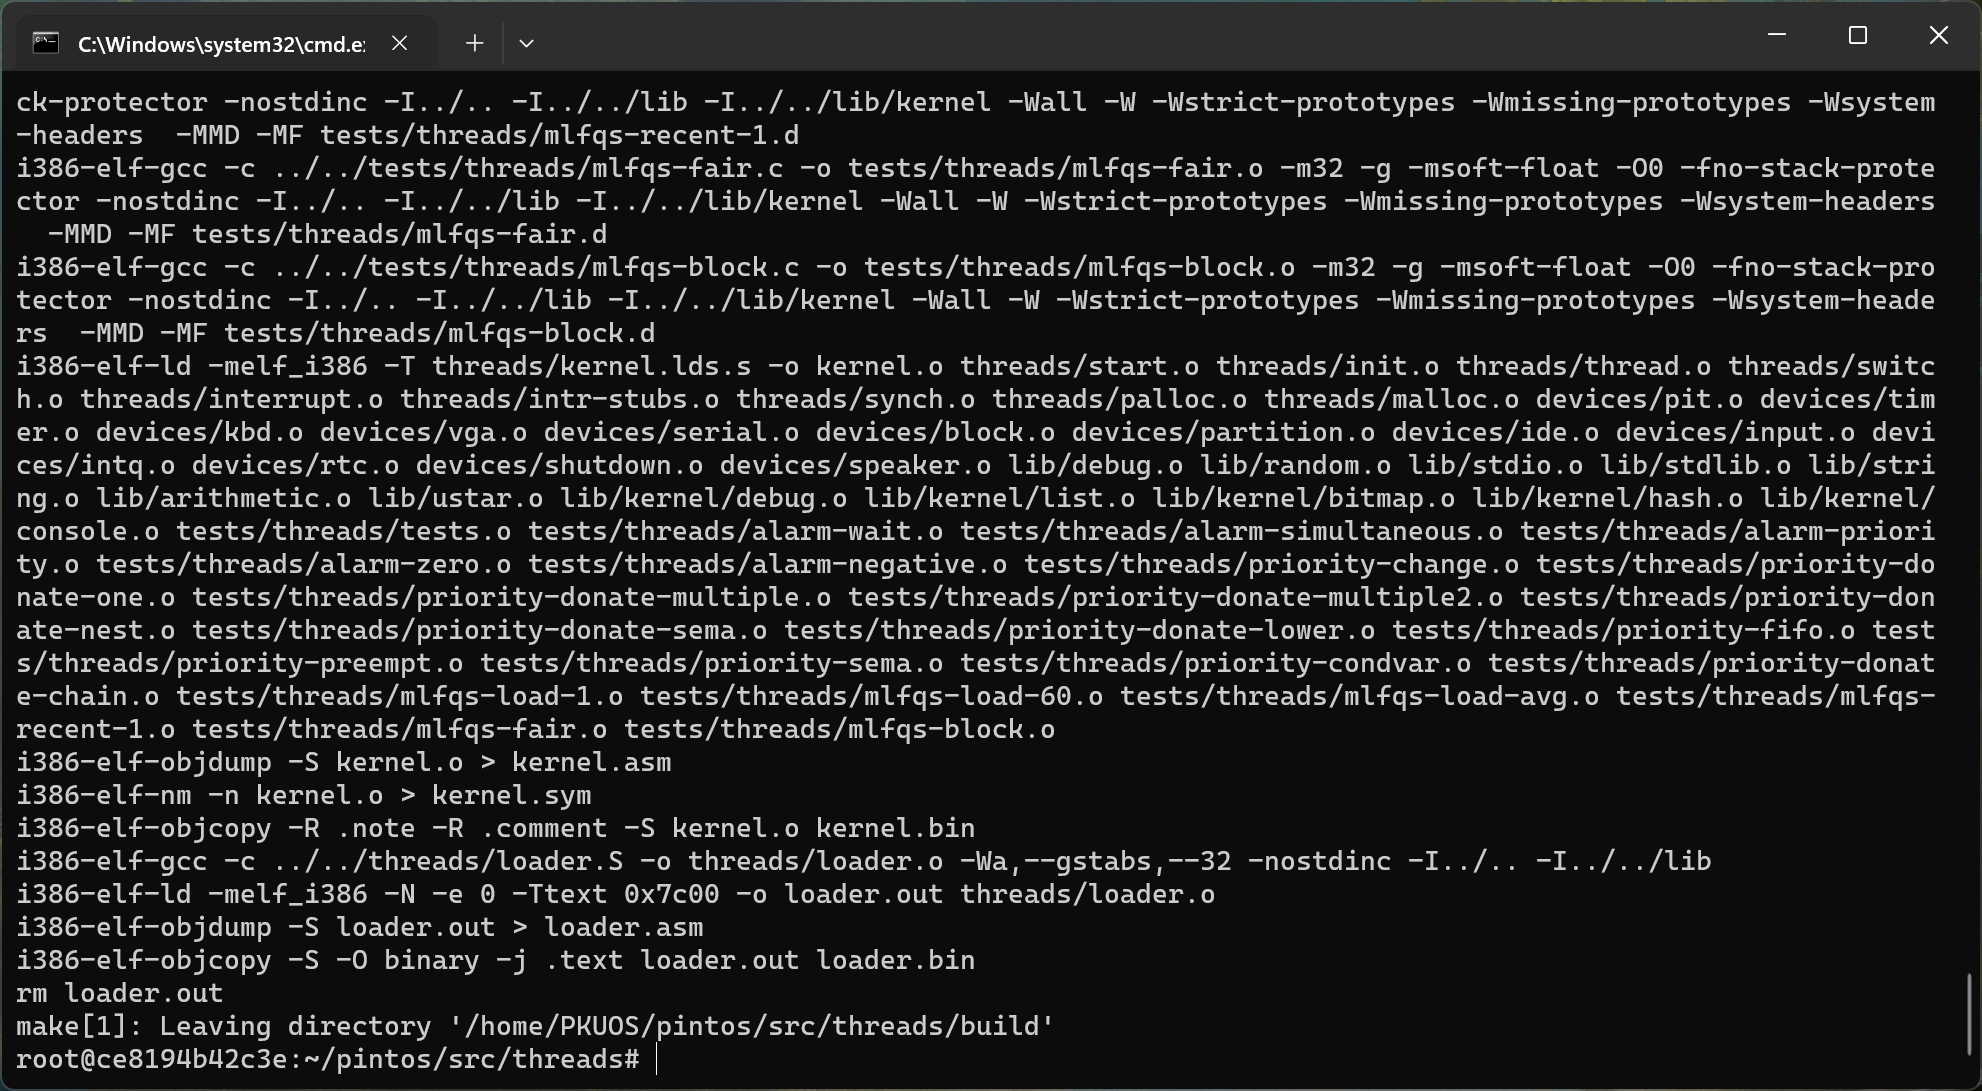
\includegraphics[width=0.6\textwidth]{img1/Make.png}
  \caption{编译Pintos}
  \label{fig:make}
\end{figure}

通过观察可以发现,输出结果中提示,此时已经离开了build目录。

\subsection{运行Pintos}
\begin{lstlisting} [language = bash, title = {运行Pintos}]
  > pintos --
\end{lstlisting}

输入该命令,输出的提示信息如下,代表 Boot 已完成,Pintos 已成功编译。

\begin{figure} [H]
  \centering
  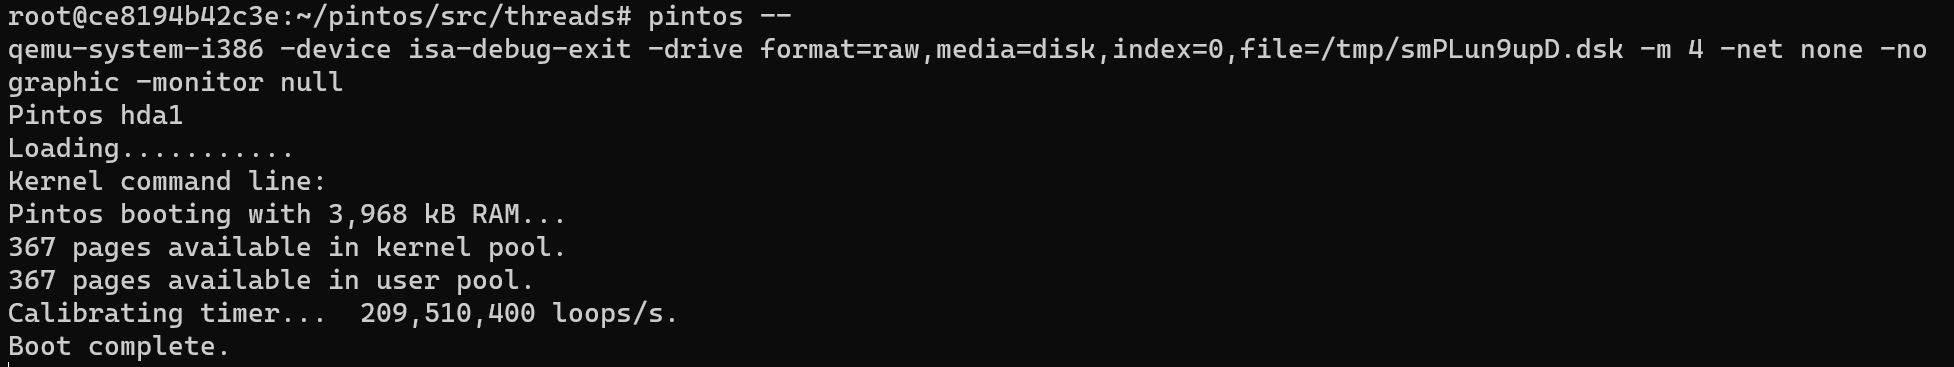
\includegraphics[width=0.6\textwidth]{img1/Boot.png}
  \caption{运行Pintos}
  \label{fig:pintosboot}
\end{figure}

\subsection{完成alarm-multiple}

\subsubsection{进入build文件夹}

当完全 Boot 完成后,会发现终端卡在了 Boot Complete, 而没有退出回到可以交互的状态。

此时,使用 Ctrl + C 组合键打断此时的状态,然后回退到可交互的 Bash 终端中,可以发现,回退到了 \texttt{/pintos/src/thread}

通过 \texttt{ls} 指令查看当前文件夹,并且通过 \texttt{cd build} 进入 build 文件夹内

\begin{figure} [H]
  \centering
  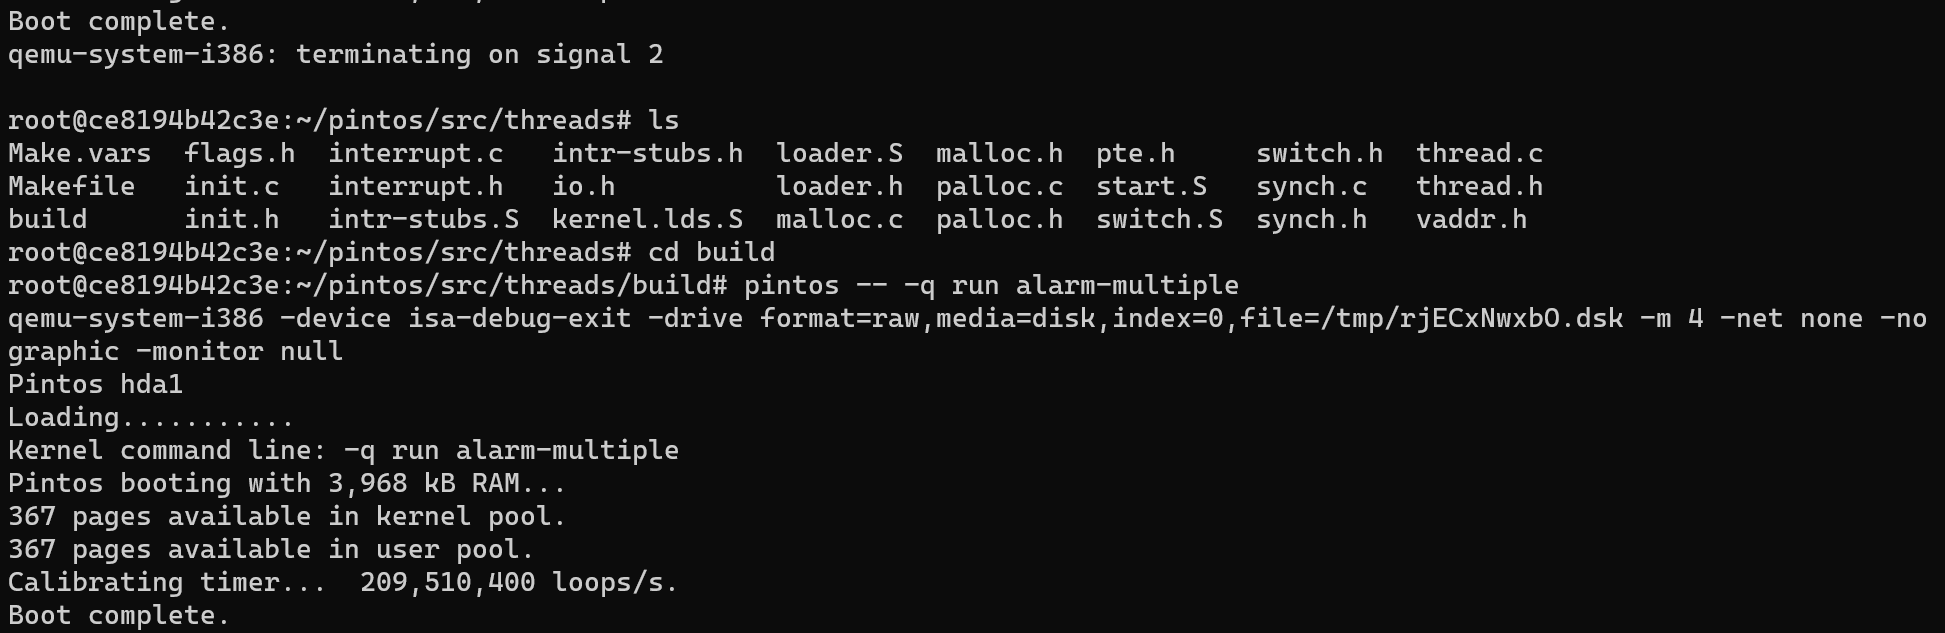
\includegraphics[width=0.6\textwidth]{img1/CtrlC.png}
  \caption{进入build文件夹}
  \label{fig:build}
\end{figure}

\subsubsection{Run alarm-multiple}

\begin{lstlisting} [language = bash, title = {Run alarm-multiple}]
  > pintos -- -q run alarm-multiple
\end{lstlisting}

\begin{figure} [H]
  \centering  
  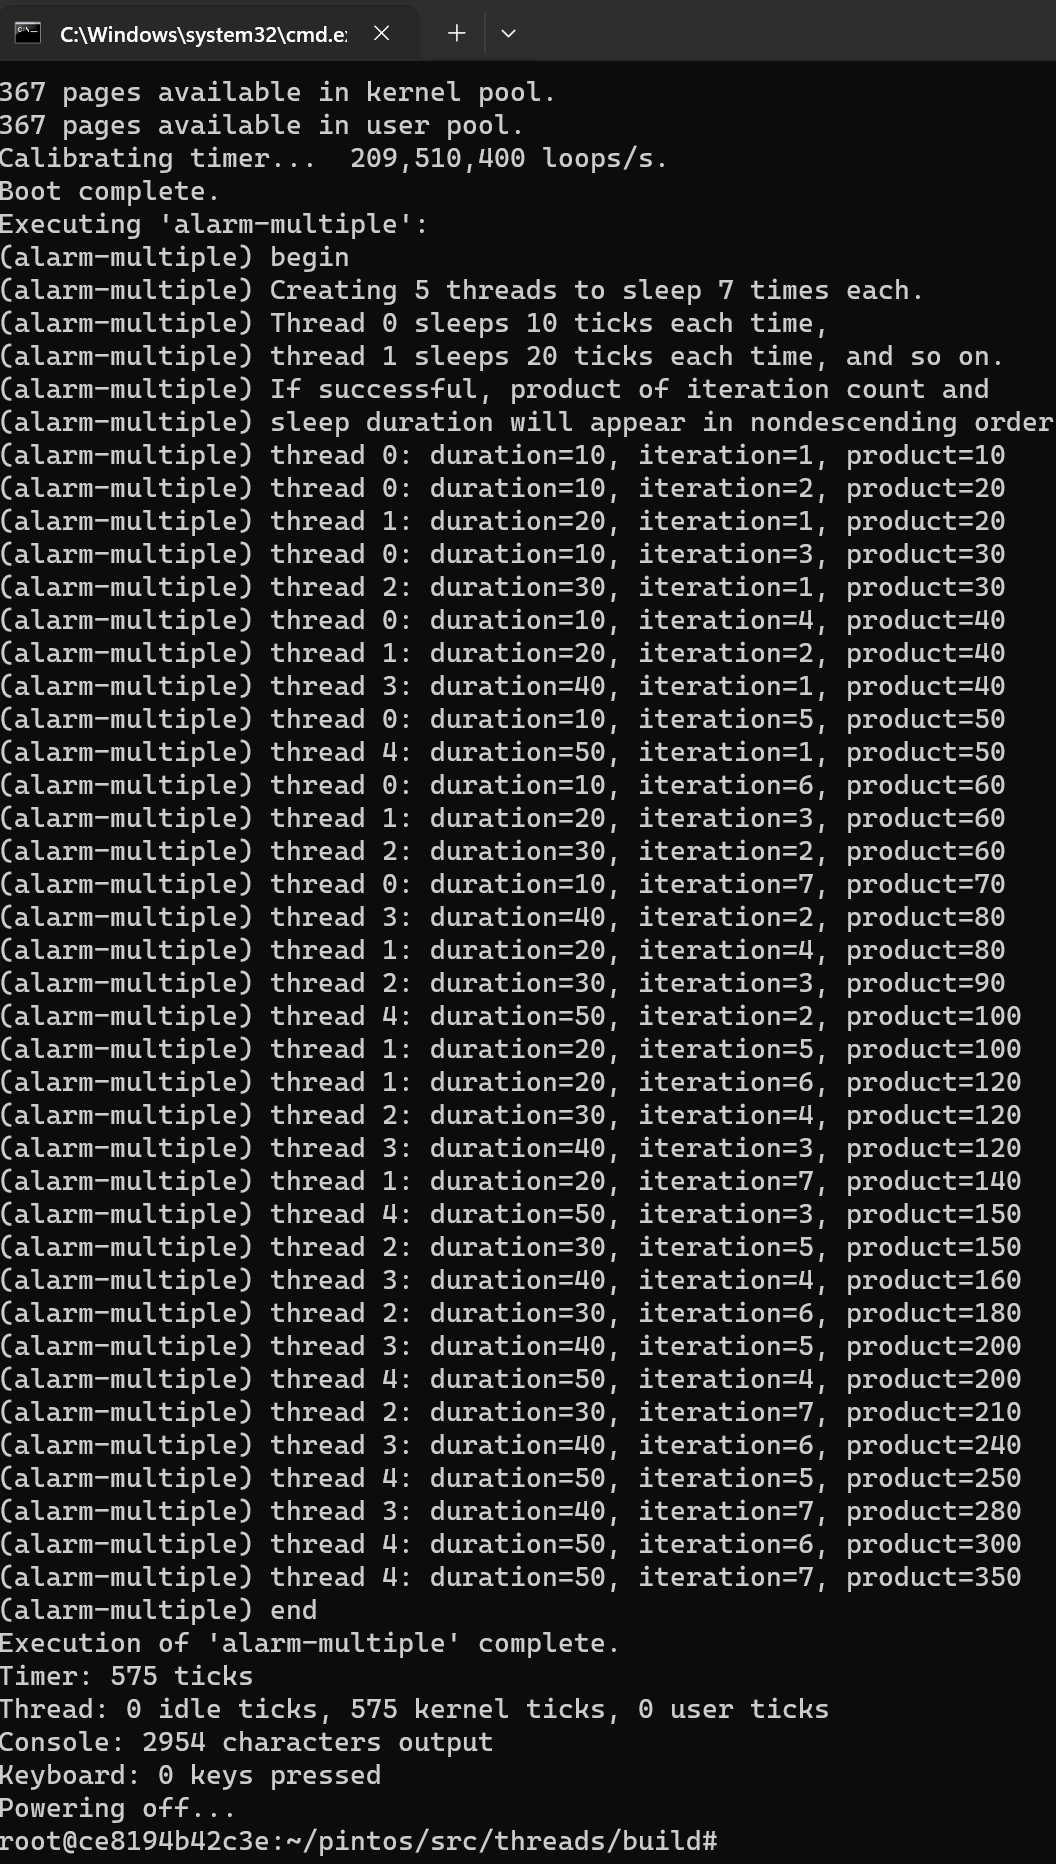
\includegraphics[width=0.5\textwidth]{img1/Alarm.png}
  \caption{运行alarm-multiple}
  \label{fig:runalarm}
\end{figure}

\subsection{实验结束,进行后续预热}

在 Docker 中的 Container 里运行时,交互的命令不是 Windows,使用的是 Exit 命令来退出当前的 Container。

\begin{itemize}
  \item \textbf{退出交互模式}:
  \begin{itemize}
      \item 使用 `exit` 命令:
      退出当前的交互终端并关闭容器(如果容器是通过交互模式启动的)。
      
      \item 使用快捷键 `Ctrl + D`:
      在没有挂起的进程时,按下 `Ctrl + D` 也会退出交互模式。
  \end{itemize}

  \item \textbf{保持容器运行并退出交互模式}:
  \begin{itemize}
      \item 使用快捷键 `Ctrl + P` 然后 `Ctrl + Q`:
      容器继续在后台运行,你可以从交互模式中分离。
      
      通过以下命令重新连接到容器:
      \begin{verbatim}
      docker attach <container_id_or_name>
      \end{verbatim}
  \end{itemize}

  \item \textbf{从宿主系统停止容器}:
  \begin{itemize}
      \item 列出所有正在运行的容器:docker ps
      \item 使用 `docker stop` 命令停止容器:
      \begin{verbatim}
      docker stop <container_id_or_name>
      \end{verbatim}
  \end{itemize}

  \item \textbf{在容器内部运行命令关闭}:
  \begin{itemize}
      \item 使用 `shutdown` 命令关闭容器内的操作系统:shutdown now
      \item 使用 `halt` 命令停止当前容器系统:
  \end{itemize}
\end{itemize}

\section{实验结果总结}

通过在虚拟机中运行的方式,无法将本地文件与 Container 内的文件相关联,于是我选择在主机上 Clone 代码,然后挂载到 Docker 中运行。

首先,Clone 代码到本地(Path: C:\\Users\\26421\\pintos)

使用如下代码将Pintos目录挂载到Docker中,以后所有的变化都会同步到本地。

\begin{lstlisting}
  docker run -it --rm --name pintos --mount type=bind,source=C:\Users\26421\pintos, target=/home/PKUOS/pintos pkuflyingpig/pintos bash
\end{lstlisting}

这一部分是参考官方文档:\href{https://pkuflyingpig.gitbook.io/pintos/getting-started/environment-setup}{\underline{https://pkuflyingpig.gitbook.io/pintos/getting-started/environment-setup}}

因为我们所有的文件更改都会同步到 Windows 系统中,所以要加入 -rm 参数告诉 Docker 每次运行结束后就删除 Container,不然会占用很多的存储空间。

\begin{figure} [H]
  \centering
  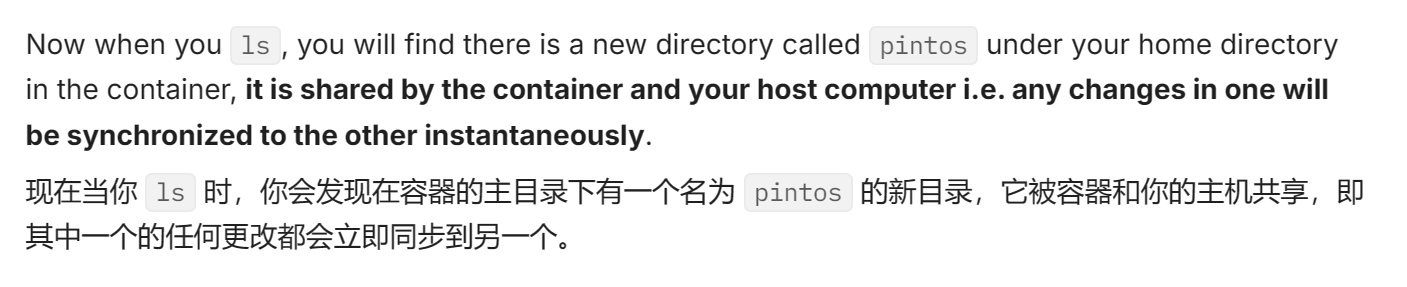
\includegraphics[width=0.6\textwidth]{img1/Shared.png}
  \caption{挂载目录}
  \label{fig:mount}
\end{figure}

\subsection{自定义 Windows 命令实现 Alias}

由于每一次我们都需要在 Windows Bash 终端中输入同样的命令以挂载到 Docker 中,所以我们可以自定义 Windows 命令,以省略每一次输入大量命令的步骤。

\subsubsection*{新建批处理文件}

新建 PintosPintos.txt 于 Windows Desktop 中,输入以下命令:

\begin{lstlisting} [language = bash, title = {PintosPintos.txt}]
  @echo off
  docker run -it --rm --name pintos --mount type=bind,source=C:\Users\26421\pintos, target=/home/PKUOS/pintos pkuflyingpig/pintos bash
\end{lstlisting}

其中,@echo off 是用来隐藏批处理文件执行时的命令行输出,只显示实际的执行结果,使脚本运行时的输出更加简洁明了。

之后,将这个文本文件重命名为 Pintos.bat,当桌面目录添加至系统的环境变量 PATH 中,于是使用 Win + R,输入 cmd,再输入 Pintos.bat 即可运行 Pintos 容器。

\section{附录}

本实验参考了以下资源:
\begin{itemize}
  \item PKU-OS 文档:\href{https://pkuflyingpig.gitbook.io/pintos/getting-started/environment-setup}{\underline{https://pkuflyingpig.gitbook.io/pintos/getting-started/environment-setup}}
  \item Docker 官方文档:\href{https://docs.docker.com/}{\underline{https://docs.docker.com/}}
\end{itemize}

\end{document}